\chapter{Detailed information on home-made lowpass filters}
\clearpage
\section{Low-pass RC filter components}\label{app:lowpassfilter}

For an overview of the different types of lumped frequency filters, for example to design a filter with a different cut-off frequency, we refer the reader to the OKAWA Electric design calculators\footnote{\url{http://sim.okawa-denshi.jp/en/Fkeisan.htm}}.
%
The low-pass filters used in this thesis consist of two-stage RC filters, cf. Fig.~\ref{fig:rctwostage} with the following values:
%
$R_1=\SI{470}{\ohm}$\footnote{Farnell 121-5922 MMU01020C4700FB300 - Surface Mount MELF Resistor, \SI{470}{\ohm}, MMU 0102 Series, \SI{100}{V}, Metal Film, \SI{100}{\milli\watt}, $\pm\SI{1}{\percent}$}, $R_2=\SI{2}{\kilo\ohm}$\footnote{Farnell 171-7632 ERA6ARB202V - SMD Chip Resistor, 0805 [2012 Metric], \SI{2}{\kilo\ohm}, ERA6A Series, \SI{100}{V}, Metal Film, 125 mW}\footnote{Farnell 121-5939 MMU01020C2001FB300 - Surface Mount MELF Resistor, \SI{2}{\kilo\ohm}, MMU 0102 Series, \SI{100}{V}, Metal Film, \SI{200}{\milli\watt}, $\pm\SI{1}{\percent}$ (these are round ones)}, $C_1=\SI{10}{\nano\farad}$\footnote{Farnell 882-0074 GRM2195C1H103JA01D - SMD Multilayer Ceramic Capacitor, \SI{10000}{\pico\farad}, \SI{50}{V}, 0805 [2012 Metric], $\pm\SI{5}{\percent}$, C0G / NP0, GRM Series}, $C_2=\SI{470}{\pico\farad}$\footnote{Farnell 180-0825 C0805C471J2GACTU - SMD Multilayer Ceramic Capacitor, \SI{470}{\pico\farad}, \SI{200}{V}, 0805 [2012 Metric], $\pm\SI{5}{\percent}$, C0G / NP0}.
%
The connectors for the filter PCBs can also be bought on Farnell\footnote{134-2652 19-70-1-TGG - RF / Coaxial Connector, SMA Coaxial, Edge Launch Jack, Solder, 50 ohm, Beryllium Copper}.
%
Our PCBs require surface mount devices of type \textbf{0805} or \textbf{2012 metric}.

When ordering, care needs to be taken on the resistor type:
%
There are \textit{thin/metal} and \textit{thick film} resistors.
%
Resistors of type \textit{thick film} should not be used, as they typically use Ruthenium oxide as resistive film with a large temperature coefficient.
%
Hence, once cooled to lower temperatures, these resistors will dramatically change resistance.
%
Instead, we use \textit{thin film} or \textit{metal electrode leadless faces} (MELF) resistors.
%
These have a very low temperature coefficient, so they are much more stable.
%
MELF resistors are cylindrical, so assembling them can be tricky since they easily roll away, but typically have higher voltage and power ratings.

There are also different types of SMD capacitors.
%
The ones used in this thesis are of type \textit{C0G (NP0)} dielectric, which provide high-quality temperature stability.
%
SMD capacitors rated \textit{GCM} (automotive grade) are to be preferred over \textit{GRM} (general purpose), as they have a higher reliability rating, which is especially important for cryogenic experiments.

To assemble the lowpass filters, we apply solder paste to the metal pads of our PCBs at \textit{DEMO} at TU Delft, place the SMD elements on the necessary locations, and either cure the solder paste using a heat gun or a dedicated oven.
%
The connectors are subsequently soldered on using a standard solder iron.

\begin{figure}
	\centering
	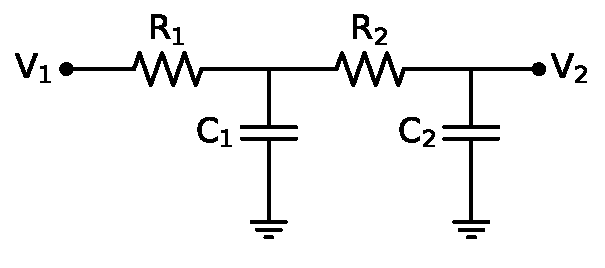
\includegraphics[width=.5\linewidth]{appendix/figs/RC_twostage}
	\caption{
		\textbf{Circuit schematic of a two-stage lowpass RC filter.}
	}
	\label{fig:rctwostage}
\end{figure}

\section{Copper powder filters}\label{app:copperpowder}

We here provide the detailed recipe we used to make our own copper-powder filters, based on a recipe shared with us by Jason Mensingh at QuTech, Delft.
%
These filters usually consist of a long meandering transmission line on a PCB connectorized with SMA connectors and encased in a copper box.
%
To suppress high-frequency radiation above \SI{1}{\giga\hertz}, the box is then filled with copper powder epoxy.
%
Due to the chemical nature of this process, it is highly recommended to do all of this in a fumehood in a chemical lab and to follow standard laboratory procedures.

\subsection{Ingredients and tools}
\begin{itemize}
	\item Resin-hardener epoxy combination \textit{Poly-Pox injecteerhars}\footnote{\url{https://www.polyservice.nl/epoxyhars-sets/374-poly-pox-injecteerhars.html?search_query=injecteer&results=8}}
	%
	\begin{itemize}
		\item \SI{200}{\gram} resin (\textit{hars})
		%
		\item \SI{100}{\gram} hardener (\textit{harder})
	\end{itemize}
	%
	\item Copper powder from SigmaAldrich\footnote{Copper powder (spheroidal), \SIrange{10}{25}{\micro\meter}, \SI{98}{\percent}, Product no. 326453, CAS 7440-50-8, \url{https://www.sigmaaldrich.com/catalog/product/aldrich/326453?lang=en&region=NL}}
	%
	\item (TU Delft) paper coffee cup
	%
	\item BD Plastikpak \SI{2}{\milli\liter} syringe 300185\footnote{\url{https://www.lab-shop.co.uk/liquid-handling-4597/plastipak-sterile-disposable-syringes-4469/plastipak-300185-sterile-disposable-425054.htm}}
	%
	\item KimtechScience small wipes 05511\footnote{\url{http://www.kcprofessional.com/en-us/products/wipers/specialty-wipers/05511}}
	%
	\item HUBY-340 cotton swabs\footnote{\url{http://www.cleancross.net/english/products/threeinch_slim.html\#BB-001}}
	%
	\item spatula
	%
	\item scissors
	%
	\item precision scale
\end{itemize}

\begin{figure}
	\centering
	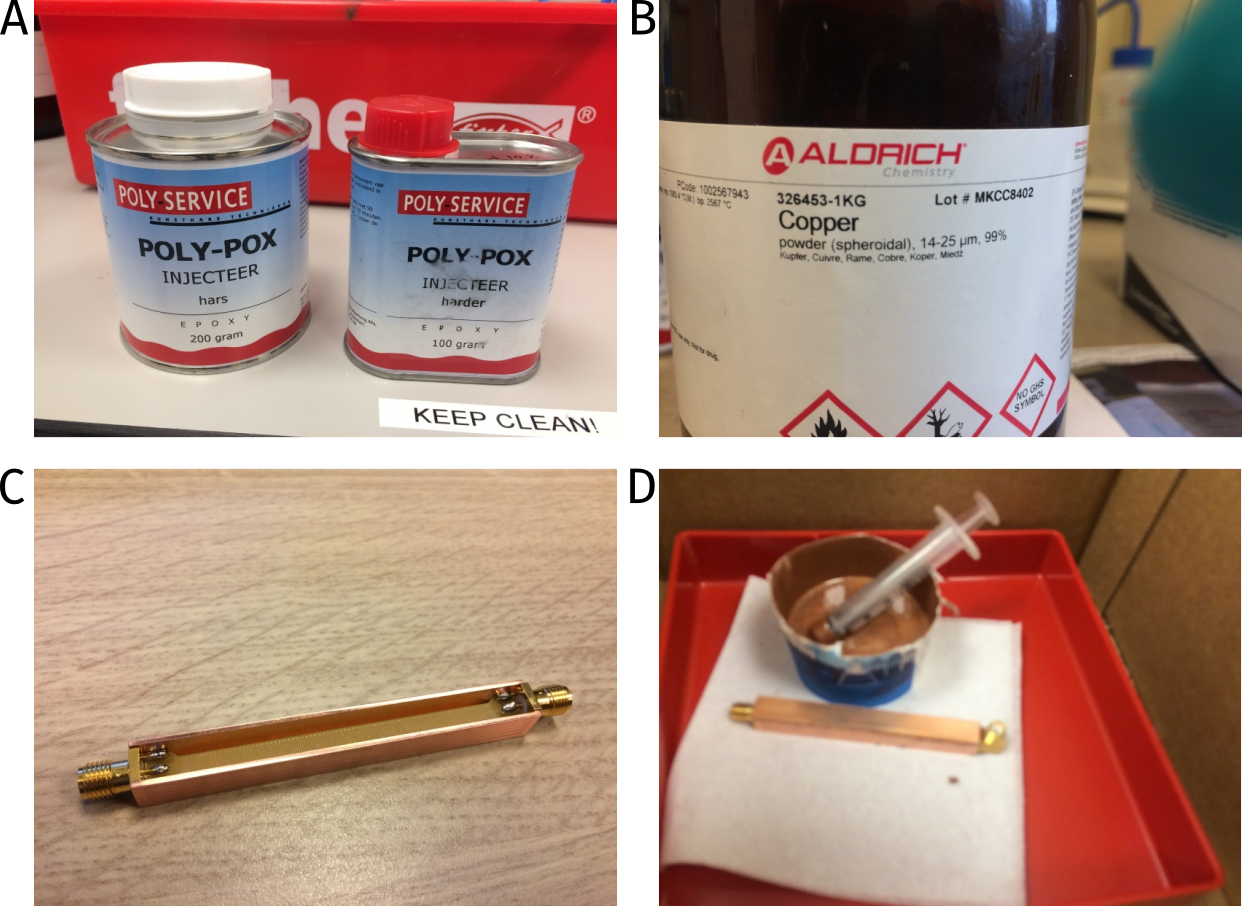
\includegraphics[]{{appendix/figs/copperpowderfilterrecipe.svg}.png}
	\caption{
		\textbf{Making copper powder filters.}
		%
		\textbf{A,} Resin and hardener from \textit{POLY-SERVICE}.
		%
		\textbf{B,} Copper powder from \textit{SigmaAldrich}.
		%
		\textbf{C,} PCB with soldered SMA connectors, inside the bottom part of its copper housing.
		%
		\textbf{D,} Dried copper powder mixture, together with a finished copper powder filter.
	}
	\label{fig:copperpowderfilterrecipe}
\end{figure}

\subsection{Instructions}
\begin{itemize}
	\item Fill \SI{10}{\gram} resin into the coffee cup and add \SI{5}{\gram} hardener
	%
	\item Stir for a few minutes using the spatula.
	%
	The mixture should be slightly yellow, clear and very liquid.
	%
	Bubbles are normal.
	%
	\item Carefully, and in the fumehood add \SI{79.5}{\gram} copper powder.
	%
	The total weight should read \SI{94.5}{\gram}
	%	
	\item Stir again for a few minutes, until there are no more visible grains, also in the edges of the cup.
	%
	The mixture should look like quite viscous liquid Nutella.
	%
	\item At this point it is safe to work outside of the fume hood.
	%
	Cut down the walls of the coffee cup using the scissors.
	%
	This will make it easier to fill the syringe.
	%
	\item Fill the syringe from the cup. 
	%
	One syringe should be enough for one of our usual rectangular copper boxes.
	%
	\item Slowly squirt the mixture into the copper box.
	%
	Be careful, as the epoxy has very low viscosity!
	%
	Slightly overfill the box.
	%
	\item Put the lid on and press it onto the bottom piece. Then, using the swab, clean off spilled-over epoxy.
	%
	\item Leave the rest of the mixture with the syringe next to the copper powder filter box for about a day.
	%
	The next day, if the mixture inside the cup is solid, then it will also be solid inside the box.
	%
	This is because the epoxy is hardened through a chemical reaction, not evaporation.
\end{itemize}

\subsection{Testing the filter}
\begin{itemize}
	\item Measure the filter resistance using a handheld multimeter.
	%
	Typical through-resistance is around \SI{3}{\ohm}, while center pin to ground should be open.
	%
	\item Connect the filter to a VNA and measure the transmission using cryocompatible cables at RT.
	%
	\item Dunk the filter into liquid nitrogen and repeat the measurements repeatedly.
	%
	\item Note that when taking the filter back out of nitrogen, the inside might be shorted to ground because of air moisture.
	%
	The readings should be back to normal after one hour.
\end{itemize}

%\clearpage
%\references{dissertation}

